En esta sección se exponen los diversos aspectos relacionados con la planificación del proyecto. Para facilitar la compresión de los datos y figuras que se van a mostrar más adelante, en la tabla \ref{tab:task_id_name}, se expone la relación entre los identificadores de las tareas y sus denominaciones.

\begin{table}[htp]
	\centering
	\caption{Relación identificador-tarea}\label{tab:task_id_name}
	\begin{tabular}{cc}
		\toprule
    	\textbf{Identificador} & \emph{Nombre}\\
    	\midrule
		T1 & Definición del problema\\
		T2 & Especificación de requisitos\\
		T3 & Especificación funcional\\
		T4 & Diseño del software\\
		T5 & Implementación\\
		T6 & Integración\\
		T7 & Adquisición de material para el Smart Mirror\\
		T8 & Validar y verificar software\\
		T9 & Creación de guía de usuario\\
    	\bottomrule
    \end{tabular}
\end{table}

\subsection{Diagrama de precedencias}

En esta sección se muestra el diagrama de precedencias (ver figura \ref{fig:network_diagram}).

\begin{figure}[!htbp]
	\centering
	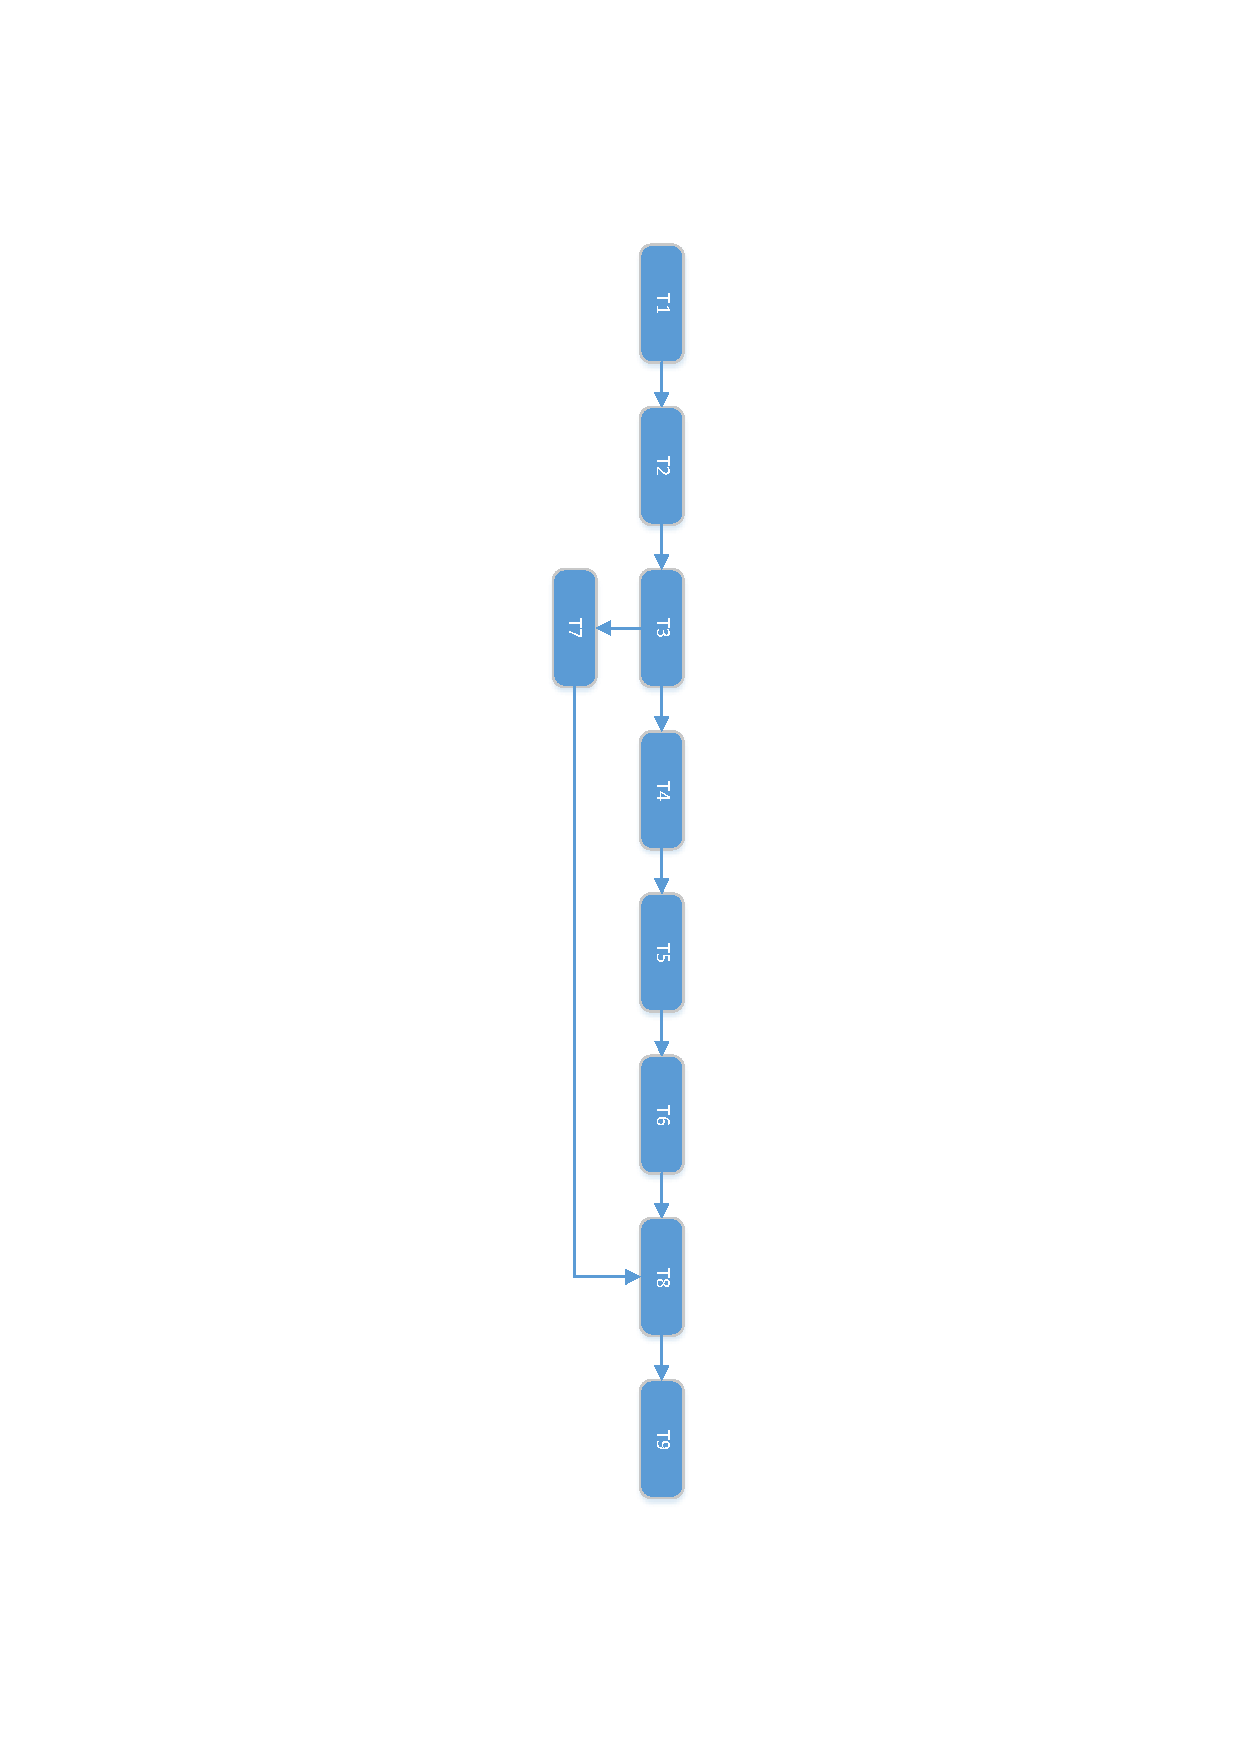
\includegraphics[page=1, scale=.8]{fig/diagrama_precedencias}
	\caption{Diagrama de precedencias}\label{fig:network_diagram}
\end{figure}